\documentclass{article}
\usepackage{graphicx}

\newcommand{\projectnaam}{Assignment: Working with Stride}
\newcommand{\student}{Johannes Akkermans}
\newcommand{\team}{
	\=Johannes Akkermans, \\\>Thomas Van Bogaert, \\\>Gilles De Borger, \\\>Siegfried Kriekemans, \\\>Zhong Xi Lu
}

\title{\textmd{\textbf{Bachelor eindwerk}}\\\normalsize\vspace{0.1in}\Large{\projectnaam}\\\vspace{0.1in}\small{\textit{3 Ba INF \  2017-2018}}}
\author{}

\begin{document}
\maketitle

\begin{center}
	\parbox{0cm}{
		\begin{tabbing}
		\textbf{Group:} \team
		\end{tabbing}
	}
\end{center}

\newpage
\section{Assignment}
\begin{center}
	\textit{Investigate the influence of R0 on the attack rate.}
\end{center}

\section{Solution}
Om het verband te bepalen tussen de R0 en de attack rate is er 10 maal een simulatie gedaan die allen 10 dagen draait met verschillende waardes voor R0. Hiervoor zijn de waardes $R0 \in \{0,1,2,3,4,5,6,7,8,9\}$ genomen.

Met behulp van de \texttt{pystride} worden de 10 verschillende forks gesimuleerd en de resultaten zijn vervolgens te vinden in de \texttt{simulations} folder in de verschillende \texttt{summary.csv} bestanden. 

Hieronder zal er een overzicht gegeven worden van de verschillende attack rates bij de desbetreffende R0-waarde.

\begin{table}[h]
	\centering
	\begin{tabular}{ | l | r | }
		\hline			
		\textbf{R0} & \textbf{Attack Rate}  \\ \hline
		0 & 0.002  \\
		1 & 0.00212  \\
		2 & 0.00222167  \\
		3 & 0.00233833  \\
		4 & 0.00242  \\
		5 & 0.00255333  \\
		6 & 0.002655  \\
		7 & 0.00273  \\
		8 & 0.002865  \\
		9 & 0.00294  \\
		\hline  
	\end{tabular}
	\caption{Results of the simulation}
\end{table}

Als de bovenstaande waardes worden weergegeven in een grafiek, lijkt het erop dat er in dit geval een positief lineair verband bestaat tussen de R0 en de attack rate.

\begin{figure}[h]
	\centering
	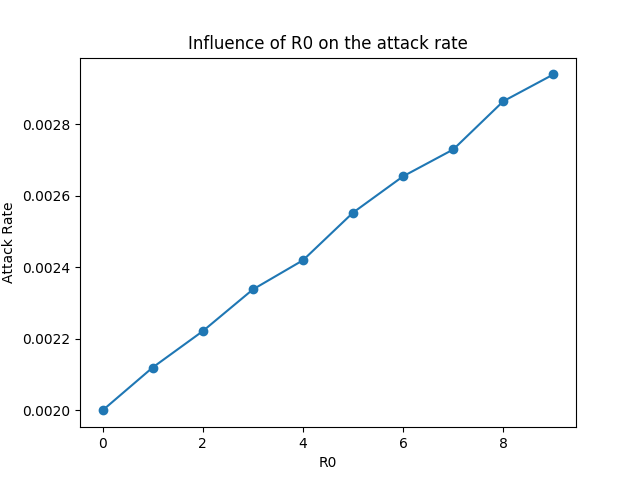
\includegraphics[width=0.5\textwidth]{r0}
	\caption{Results of the simulation in a graph}
\end{figure}





\end{document}